\documentclass[10pt,a4paper,twocolumn]{article}

\usepackage[T1]{fontenc}
\usepackage[utf8]{inputenc}
\usepackage{lmodern}
\usepackage{textcomp}
\usepackage[margin=0.85in]{geometry}
\setlength{\columnsep}{18pt}
\usepackage{microtype}
\usepackage{booktabs}
\usepackage{tabularx}
\usepackage{longtable}
\usepackage{caption}
\usepackage{listings}
\usepackage{xcolor}
\usepackage{enumitem}
\usepackage{titlesec}
\usepackage{fancyhdr}
\pagestyle{fancy}
\fancyhf{}
\fancyhead[L]{\small\itshape Neo4j: A Native Property Graph Database}
\fancyhead[R]{\small Team 6}
\fancyfoot[C]{\thepage}
\renewcommand{\headrulewidth}{0.4pt}
\setlength{\headheight}{14pt}
\usepackage{tikz}
\usetikzlibrary{positioning,arrows.meta}
\usepackage[hidelinks]{hyperref}
\usepackage{url}
\Urlmuskip=0mu plus 1mu
\def\UrlBreaks{\do\/\do-\do.\do_\do?\do\&\do=}

% --- listings style for SQL / Cypher -----------------------------------
\definecolor{codebg}{RGB}{248,249,252}
\definecolor{codeframe}{RGB}{218,222,232}
\definecolor{kw}{RGB}{28,78,168}        % keywords: blue
\definecolor{str}{RGB}{163,48,48}       % strings: brick red
\definecolor{cmt}{RGB}{110,120,132}     % comments: grey
\definecolor{num}{RGB}{22,120,90}       % numbers: green
\definecolor{ident}{RGB}{40,44,52}      % plain text
% figure palette
\definecolor{sqlblue}{RGB}{31,88,148}
\definecolor{sqlfill}{RGB}{233,241,250}
\definecolor{graphgreen}{RGB}{23,125,92}
\definecolor{graphfill}{RGB}{228,244,238}
\definecolor{relorange}{RGB}{193,104,22}

\lstdefinelanguage{Cypher}{
  morekeywords={MATCH,OPTIONAL,RETURN,WHERE,WITH,CREATE,MERGE,SET,DELETE,DETACH,REMOVE,
    DISTINCT,ORDER,BY,LIMIT,SKIP,AS,AND,OR,NOT,IN,STARTS,ENDS,CONTAINS,UNWIND,CALL,YIELD,
    CONSTRAINT,INDEX,FOR,REQUIRE,UNIQUE,ASC,DESC,NULL,TRUE,FALSE},
  morekeywords=[2]{count,date,time,length,duration,collect,avg,sum,min,max,toInteger,size},
  sensitive=false,
  morestring=[b]',
  morecomment=[l]{//},
}
\lstdefinestyle{query}{
  basicstyle=\ttfamily\footnotesize\color{ident},
  backgroundcolor=\color{codebg},
  keywordstyle=\color{kw}\bfseries,
  keywordstyle=[2]\color{num},
  stringstyle=\color{str},
  commentstyle=\color{cmt}\itshape,
  numberstyle=\color{num},
  frame=single,
  rulecolor=\color{codeframe},
  framerule=0.4pt,
  breaklines=true,
  breakatwhitespace=false,
  columns=fullflexible,
  keepspaces=true,
  showstringspaces=false,
  xleftmargin=6pt,
  xrightmargin=6pt,
  aboveskip=8pt,
  belowskip=8pt,
}
\lstdefinestyle{sqlcode}{style=query,language=SQL}
\lstdefinestyle{cyphercode}{style=query,language=Cypher}
\lstset{style=query,captionpos=t,abovecaptionskip=4pt,belowcaptionskip=2pt}
\renewcommand{\lstlistingname}{Listing}
\renewcommand{\lstlistlistingname}{List of Listings}

\titleformat{\section}{\normalfont\Large\bfseries}{\thesection}{1em}{}
\titleformat{\subsection}{\normalfont\large\bfseries}{\thesubsection}{1em}{}

\setlist[itemize]{itemsep=2pt,topsep=4pt}
\renewcommand{\topfraction}{0.9}
\renewcommand{\textfraction}{0.07}
\renewcommand{\floatpagefraction}{0.75}
\setcounter{topnumber}{2}

\newcolumntype{Y}{>{\raggedright\arraybackslash}X}
\newcolumntype{R}[1]{>{\raggedright\arraybackslash}p{#1}}
\captionsetup[table]{skip=4pt,font=small,labelfont=bf}

\title{\textbf{Neo4j: A Native Property Graph Database}}
\author{Rigesh Krishnaraj \and Suresh Hemal Warnasooriya Warnakulasooriya Mudiyanselage \and Scott C. Robertson}
\date{September 28, 2026}

\begin{document}

\begin{titlepage}
\centering

\vspace*{0.5cm}

{\LARGE\bfseries New Mexico State University \par}
\vspace{0.4cm}
{\large Department of Computer Science \par}

\vspace{1.2cm}

\rule{\textwidth}{0.4pt}
\vspace{0.6cm}

{\large\scshape CSCI 4140 / 5140 --- Database Management Systems \par}

\vspace{0.9cm}

{\Huge\bfseries Group Research Project \par}
\vspace{0.4cm}
{\LARGE\bfseries Phase 1 Report \par}

\vspace{0.7cm}

{\Large\itshape Neo4j: A Native Property Graph Database \par}
\vspace{0.3cm}
{\large Data Model, Query Language, and Readiness for Experimental Comparison with MySQL \par}

\vspace{0.6cm}
\rule{\textwidth}{0.4pt}

\vspace{1.4cm}

{\large\bfseries Team 6 \par}

\vspace{0.8cm}

{\large
\begin{tabular}{c}
Rigesh Krishnaraj \\[0.35cm]
Suresh Hemal Warnasooriya Warnakulasooriya Mudiyanselage \\[0.35cm]
Scott C. Robertson \\
\end{tabular}
\par}

\vfill

{\large
\begin{tabular}{rl}
\textbf{Instructor:} & Dr. Parth Nagarkar \\[0.25cm]
\textbf{Semester:}   & Fall 2026 \\[0.25cm]
\textbf{Submitted:}  & September 28th, 2026 \\
\end{tabular}
\par}

\vspace{1.2cm}

{\small Submitted in partial fulfilment of the requirements for CSCI 4140 / 5140 \par}

\vspace{0.5cm}

\end{titlepage}

\clearpage
\pagenumbering{roman}
\tableofcontents
\clearpage
\listoftables
\clearpage
\lstlistoflistings
\clearpage
\pagenumbering{arabic}

% =======================================================================
\section{Introduction}

The database in question that we chose for the Database Management Systems project is Neo4j which was created by Emil Eifrem, Johan Svensson, and Peter Neubauer in Sweden~\cite{wikipedia2026neo4j}. The company in which it was created was originally called Neo Technology and was eventually renamed to Neo4j, Inc.\ on July 27th, 2017~\cite{eifrem2017helloworld}. The name can be split into two parts. The first part, ``Neo'', means new and the second part, ``4j'' is short for ``for java''. Making the full name ``New For Java''. The project was also originally called ``Project Neo''.

Neo4j was created in 2007 along with the company in Sweden. Neo4j, was released as open source~\cite{wikipedia2026neo4j,dbdb2026neo4j}. Later on, in February 2010, the company officially released version 1.0 to the general public. In 2011, the company moved and set up shop in current Silicon Valley, California, and they kept their engineering process in Sweden~\cite{wikipedia2026neo4j,dbdb2026neo4j}.

The idea of Neo4j started off in the year 2000, while on a flight to Mumbai, where Eifrem sketched the first property graph of the now Neo4j on a napkin. The three founders at the time were building an enterprise content management system (ECM) and kept going against the challenge of using an RDBMS for querying connected data. Before the idea of Neo4j, Eifrem was originally at Windh Technologies, which is a media asset company~\cite{baer2019eifrem}.

The core idea of the company is to store relationships as first class entities instead of rebuilding them with joins~\cite{dbdb2026neo4j}. The company has its roots in Malmö, Sweden where development still occurs. Today, their headquarters is in San Mateo, California~\cite{oresund2016neo}.

% =======================================================================
\section{Data Model Fit}

\subsection{Background: Data Models in the DBMS Landscape; A Brief Introduction}

Table~\ref{tab:models} groups non-relational data into eight different categories~\cite{stonebraker2024whatgoesaround}, together with the relational model for comparison.

\begin{table*}[tbp]
\centering\footnotesize
\caption{Non-relational data models grouped into categories, after Stonebraker and Pavlo~\cite{stonebraker2024whatgoesaround}.}\label{tab:models}
\begin{tabular}{@{}R{0.16\linewidth} R{0.24\linewidth} R{0.21\linewidth} R{0.29\linewidth}@{}}
\toprule
\textbf{Model} & \textbf{Shape of Data} & \textbf{Examples} & \textbf{Paper's View} \\
\midrule

Relational (RM) & Tables of rows and columns, queried with SQL & MySQL, PostgreSQL, Oracle & Dominant; most other models converge back towards it \\
\addlinespace
MapReduce & No fixed model; user-written Map and Reduce functions over files & Google MR, Hadoop & ``Hadoop died about a decade ago''; replaced by Spark, Flink \\
\addlinespace
Key/value & (key, value); value is an opaque blob; get/set/delete & Memcached, Redis, DynamoDB, RocksDB & Good for caching and sessions; ``a bad idea'' when records need multiple fields \\
\addlinespace
Document & Nested field/value hierarchies (JSON) & MongoDB & Nearly all added SQL and ACID; ``will soon be effectively identical'' to RDBMSs \\
\addlinespace
Column-family (wide-column) & Records keyed by ID with optional attributes; one level of nesting & BigTable, Cassandra, HBase & Niche; lacks joins and secondary indexes \\
\addlinespace
Text search & Inverted indexes over tokenized words & Elasticsearch, Solr (Lucene) & Limited transactions; RDBMSs now offer full-text search \\
\addlinespace
Vector & One-dimensional embeddings for similarity search & Pinecone, Milvus, Weaviate & RDBMSs are quickly adding vector indexes \\
\addlinespace
Graph & Nodes and edges & Neo4j, TigerGraph, JanusGraph & ``We do not expect specialized graph DBMSs to be a large market'' \\
\bottomrule
\end{tabular}
\end{table*}


There are two ways of representing graphs~\cite{stonebraker2024whatgoesaround}:

\begin{itemize}
  \item RDF (triplestores): a directed graph with labeled edges only (subject \textrightarrow{} predicate \textrightarrow{} object).
  \item Property graph: a directed multi-graph with key/value properties on nodes and edges. It is more common, and the paper calls it ``a superset of RDF''.
\end{itemize}

In this case, Neo4j uses the property graph model.

\subsection{Mental Model: MySQL \textrightarrow{} Neo4j (using the el\_paso\_airport schema)}

\begin{figure*}[tbp]
\centering
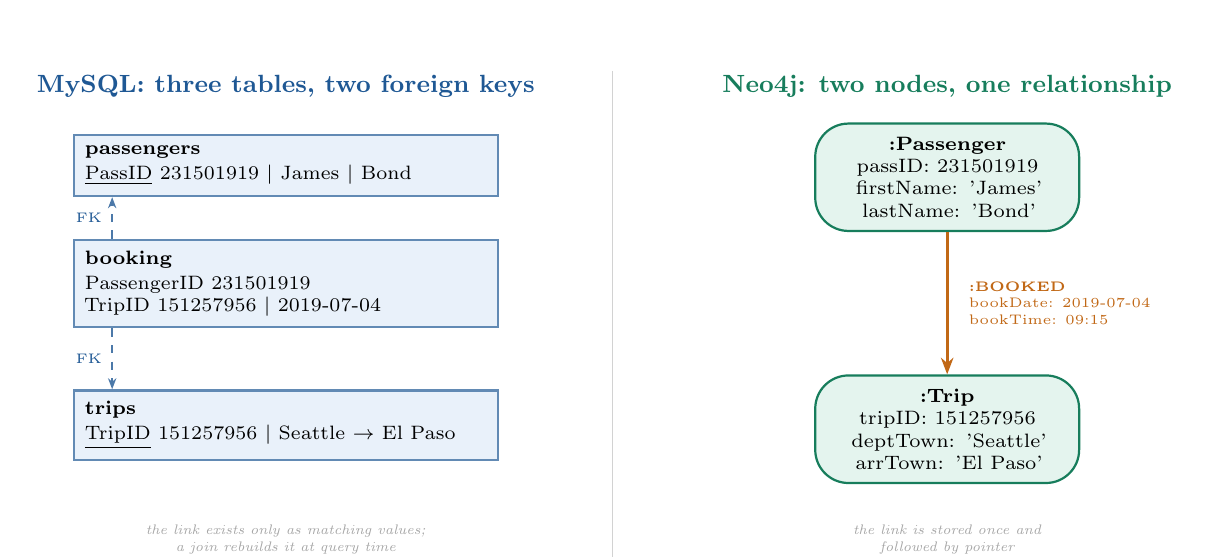
\begin{tikzpicture}[
  font=\scriptsize,
  tbl/.style={draw=sqlblue!70,thick,rectangle,align=left,inner sep=4pt,fill=sqlfill,text width=5.1cm},
  hdr/.style={font=\small\bfseries}, lhdr/.style={font=\small\bfseries,sqlblue}, rhdr/.style={font=\small\bfseries,graphgreen},
  gnode/.style={draw=graphgreen,thick,rounded corners=12pt,align=center,inner sep=5pt,text width=3.0cm,fill=graphfill},
  fk/.style={-{Stealth[length=4pt]},dashed,sqlblue!80,thick},
  rel/.style={-{Stealth[length=6pt]},very thick,relorange},
  note/.style={font=\tiny\itshape,gray!70,align=center},
]
\node[lhdr] (lt) at (0,3.0) {MySQL: three tables, two foreign keys};
\node[tbl] (pass) at (0,2.0)
  {\textbf{passengers}\\[1pt] \underline{PassID} 231501919 $\vert$ James $\vert$ Bond};
\node[tbl] (book) at (0,0.5)
  {\textbf{booking}\\[1pt] PassengerID 231501919\\ TripID 151257956 $\vert$ 2019-07-04};
\node[tbl] (trip) at (0,-1.3)
  {\textbf{trips}\\[1pt] \underline{TripID} 151257956 $\vert$ Seattle $\to$ El Paso};
\draw[fk] ([xshift=0.5cm]book.north west) -- ([xshift=0.5cm]pass.south west)
      node[midway,left,font=\tiny,sqlblue] {FK};
\draw[fk] ([xshift=0.5cm]book.south west) -- ([xshift=0.5cm]trip.north west)
      node[midway,left,font=\tiny,sqlblue] {FK};
\node[note] at (0,-2.75) {the link exists only as matching values;\\ a join rebuilds it at query time};

\node[rhdr] (rt) at (8.4,3.0) {Neo4j: two nodes, one relationship};
\node[gnode] (p) at (8.4,1.85) {\textbf{:Passenger}\\ passID: 231501919\\ firstName: 'James'\\ lastName: 'Bond'};
\node[gnode] (t) at (8.4,-1.35) {\textbf{:Trip}\\ tripID: 151257956\\ deptTown: 'Seattle'\\ arrTown: 'El Paso'};
\draw[rel] (p) -- (t);
\node[right,align=left,font=\tiny,relorange] at (8.55,0.25)
  {\textbf{:BOOKED}\\ bookDate: 2019-07-04\\ bookTime: 09:15};
\node[note] at (8.4,-2.75) {the link is stored once and\\ followed by pointer};

\draw[gray!35] (4.15,3.2) -- (4.15,-3.1);
\end{tikzpicture}
\caption{One booking, stored two ways. In MySQL the connection between a passenger and a trip lives in the \texttt{booking} table as two foreign-key values that a join must match at query time. In Neo4j the same connection is a stored \texttt{:BOOKED} relationship that carries its own properties and is followed directly.}
\label{fig:tables-vs-graph}
\end{figure*}



Figure~\ref{fig:tables-vs-graph} shows the same booking stored both ways, and Table~\ref{tab:mapping} summarizes how each MySQL concept maps onto Neo4j. In one line: labels are like table names, except a node can have several; a relationship is a foreign key or a pivot-table row promoted to a real object that can carry its own columns.

\begin{table*}[tbp]
\centering\footnotesize
\caption{Mapping of MySQL concepts to Neo4j concepts, using the el\_paso\_airport schema.}\label{tab:mapping}
\begin{tabular}{@{}R{0.30\linewidth} R{0.33\linewidth} R{0.27\linewidth}@{}}
\toprule
\textbf{MySQL} & \textbf{Neo4j} & \textbf{Note} \\
\midrule

Table name (pilots) & Label (:Pilot) & A node may have zero or more labels~\cite{neo4j2026graphdb}. \\
\addlinespace
Row & Node & \\
\addlinespace
Column & Property & Property lives on nodes and relationships~\cite{neo4j2026graphdb}. \\
\addlinespace
Foreign key column (trips.AirCraftID) & Relationship (:Trip)-[:USES]->(:Aircraft) & A single FK becomes a relationship too, not only pivot tables. \\
\addlinespace
Pivot table without extra columns (flies) & Relationship (:Pilot)-[:FLIES]->(:Trip) & The table disappears entirely. \\
\addlinespace
Pivot table with extra columns (works(StaffID, DepartmentID, Year)) & (:Staff)-[:WORKS\_IN \{year: 2019\}]->(:Department) & Extra columns become relationship properties. \\
\addlinespace
booking(PassengerID, TripID, BookDate, BookTime) & (:Passenger)-[:BOOKED \{bookDate, bookTime\}]->(:Trip) & Composite PK = the relationship itself. \\
\addlinespace
Subtype tables / UNION & Multiple labels (:Person:Pilot, :Person:Staff) & MATCH (person:Person) then matches both. \\
\bottomrule
\end{tabular}
\end{table*}


As the last row of Table~\ref{tab:mapping} shows, it is worthy to note in this report that a node can carry many labels, but a relationship can have exactly one type plus a direction, a start node, and an end node~\cite{neo4j2026graphdb}. Concrete payoff in this schema: pilots and staff repeat in the same nine columns (FirstName, LastName, Birthdate, Address, Email, PhoneNumber, Gender, Salary, HiredDate) however a shared :Person label will remove that duplication and simplifies the case of staff and pilots sharing a first name, which in SQL needs a join across the two tables. When it comes to open modeling question two, if a booking needs to store its own information, (seat number, price paid, check in time, flight status, etc.) should it become its own object, a booking node between them? This is the same as the question in traditional databases of when a connecting table should become an entity of its own.

\subsection{Data Assumptions}

The data model, as stated above, is a property graph and a directed multigraph with key/value properties on both nodes and edges~\cite{neo4j2026graphdb,stonebraker2024whatgoesaround}. The building blocks in this are the following:

\begin{itemize}
  \item Node: an entity (e.g., a person). Classified by zero or more labels (e.g., :User).
  \item Relationship: a connection that must have a start node, an end node, a direction, and exactly one type (e.g., FOLLOWS).
  \item Property: key-value pairs stored on nodes and relationships.
\end{itemize}

The relationships in this are first class relationships and stored data, not rebuilt with joins at each query time~\cite{dbdb2026neo4j}. The flexible schema is not restricted to a pre-defined model and the design can change over time. The index free adjacency is each node directly references its adjacent, neighboring, nodes. Therefore, a traversal is a pointer lookup with complexity $O(1)$ compared to an index lookup with complexity $O(\log n)$ in non-native systems~\cite{stegeman2023native}. The paper compares this to CODASYL-style pointers, which is good for the traversal of long edge chains compared to an RDBMS which must do it via joins~\cite{stonebraker2024whatgoesaround}.

\subsection{Natural Applications Supporting}

A general rule of thumb is the answer is found between the records and in the connections rather than inside of them. Graph databases are useful for the following cases:

\begin{itemize}
  \item Questions about relationships between elements such as navigating hierarchies, discovering hidden connections, and network analysis (finance, retail, government)~\cite{neo4j2026graphdb}.
  \item Social networks, which includes ``likes'', ``friends-of'' and knowledge graphs~\cite{stonebraker2024whatgoesaround}.
  \item Long chains of relationships, such with many ``hops'', and such as friends of friends. The cost of a query only depends on the data it touches and not the total size of the data~\cite{stegeman2023native}.
\end{itemize}

\subsection{Struggles}

The biggest struggles are apps with any long-chain relationship queries. The paper argues that the value of Neo4j depends on whether there are enough ``long chain'' scenarios in order to justify forgoing a relational database~\cite{stonebraker2024whatgoesaround}.

A relational database is also an option that is always on the table. A graph can be stored as just nodes and edges. Furthermore, studies show that relational databases such as SQL/PGQ in DuckDB were up to ten times faster than a leading graph database~\cite{stonebraker2024whatgoesaround}. Large scale graph analytics were also a struggle and the paper specifically mentions that this is a special case that should be done in main memory with specialized data structures~\cite{stonebraker2024whatgoesaround}.

Dense nodes, also known as ``supernodes'' are nodes with many relations, which can make data retrieval expensive. The solution to this problem is to remodel the data using intermediate nodes~\cite{neo4j2026modeling}. Horizontal scaling is another problem. Splitting a connected graph across several different machines is difficult. In addition, Neo4j struggled with scalability and added property sharding in 2025 (in Infinigraph, its self-managed offering)~\cite{clark2025sharding}.

% =======================================================================
\section{Query Language and Interface}

\subsection{Query and Programming Languages}

One of the languages it supports is Cypher, which is a declarative graph query language. It was created in 2011 by Neo4j engineers as an SQL-equivalent for graph databases~\cite{neo4j2026cypher}. Neo4j also launched the openCypher initiative in October 2015~\cite{malenchino2024opencypher}.

GQL (ISO/IEC 39075) is an ISO standard query language for property graphs and it was published on April 11, 2024~\cite{malenchino2024opencypher,hare2024gql}. It is the first ISO database query language in more than 35 years, while SQL was first published in 1987. GQL incorporates many features of openCypher, GSQL, PGQL, and G-Core, and shares its Cypher-derived pattern-matching sublanguage with SQL/PGQ~\cite{hare2024gql}. Cypher also supports most mandatory GQL features and a substantial portion of the optional ones, but a few mandatory features are noticeably missing, so it is not fully conformant~\cite{neo4j2026gqlconformance}.

The official programming languages it has drivers for are Java, Python, JavaScript, .NET, and Go, which all connect over Neo4j's Bolt protocol~\cite{neo4j2026drivers}.

\subsection{SQL Support}

Neo4j does not support SQL natively, as its native language is Cypher. However, Cypher was designed to feel like and behave like SQL, so it feels similar, such as the aggregations~\cite{neo4j2026cypher}. SQL-to-Cypher translation is also an optional feature of the Neo4j JDBC driver (\texttt{enableSQL\-Translation=true}). There are limitations to this such as outer joins and mapping tables, and there is no single way to map table names to graph objects~\cite{neo4j2026sql2cypher}.

A BI Connector also lets SQL/JDBC tools, such as Tableau, read Neo4j by exposing a virtual table for each node label and each relationship. It is read only~\cite{allen2020biconnector}.

\subsection{Key Differences}

The main differences between Cypher and SQL are the following~\cite{neo4j2026cypher}.

\begin{itemize}
  \item Cypher describes the shape to find, (passenger:Passenger)-[:BOOKED]->(trip:Trip), instead of joining tables on keys.
  \item Clause order is different. SQL starts with SELECT and Cypher ends with the RETURN clause: MATCH, WHERE, RETURN.
  \item Conciseness is a big one. Cypher queries are oftentimes more concise than SQL.
  \item Variable-length paths are where Cypher succeeds. The query in Cypher is (*1..10) where in SQL it is recursive.
  \item The paper's view is plain ``vanilla'' SQL is not expressive enough for graph queries, but SQL:2023 added SQL/PGQ, which helps further narrow functionality differences between relational and native graph databases~\cite{stonebraker2024whatgoesaround}.
\end{itemize}

\subsection{Worked Examples: el\_paso Airline Database (MySQL) vs Neo4j (Cypher)}

The SQL below comes from an earlier coursework exercise on this schema and was run against the live el\_paso\_airport database (MySQL 8.4); the Cypher gives the equivalent formulation in Neo4j.

The actual schema of el\_paso\_airport, verified with DESCRIBE, and the dataset size are given in Table~\ref{tab:schema}.

\begin{table*}[tbp]
\centering\footnotesize
\caption{The el\_paso\_airport schema and dataset size, verified with DESCRIBE (MySQL 8.4).}\label{tab:schema}
\begin{tabular}{@{}R{0.12\linewidth} R{0.72\linewidth} r@{}}
\toprule
\textbf{Table} & \textbf{Key Columns} & \textbf{Rows} \\
\midrule

aircrafts & AircraftID, Name, NumSeats, ManufacturedDate, LastServiceDate & 20 \\
booking & PassengerID + TripID (composite PK), BookDate, BookTime & 500 \\
departments & DeptID, Name, Category & 7 \\
flies & PilotID + TripID (composite PK) & 200 \\
passengers & PassID, FirstName, LastName, Birthdate, Address, Email, PhoneNumber, RewardPoints, Citizenship, Gender & 50 \\
pilots & PilotID, FirstName, LastName, Birthdate, \ldots, Salary, HiredDate, Rating & 20 \\
services & ServiceID, StaffID, Staff2ID, AirCraftID, ServiceDate, Description & 100 \\
staff & StaffID, FirstName, LastName, \ldots, Salary, DepartmentID, HiredDate, PositionName & 20 \\
trips & TripID, AirCraftID, Capacity, DeptTown, DeptDate, DeptTime, ArrTown, ArrDate, ArrTime, Fare & 200 \\
works & StaffID + DepartmentID (composite PK), Year & 20 \\
\bottomrule
\end{tabular}
\end{table*}


As the row counts in Table~\ref{tab:schema} show, this dataset is small, with at most 500 rows in any table, so it illustrates how each language expresses a question rather than how the two systems perform.

Listing~\ref{lst:model} gives the graph model for the same data, with one node per entity and one relationship per join table.

\begin{lstlisting}[caption={Property graph model for the el\_paso\_airport data},label={lst:model}]
(:Passenger {passID, firstName, lastName, birthdate, email, phoneNumber, rewardPoints, citizenship, gender})
(:Trip {tripID, capacity, deptTown, deptDate, deptTime, arrTown, arrDate, arrTime, fare})
(:Pilot {pilotID, firstName, lastName, birthdate, phoneNumber, salary, hiredDate, rating})
(:Staff {staffID, firstName, lastName, birthdate, phoneNumber, salary, hiredDate, positionName})
(:Department {deptID, name, category})
(:Aircraft {aircraftID, name, numSeats, manufacturedDate, lastServiceDate})
(:Service {serviceID, serviceDate, description})

(:Passenger)-[:BOOKED {bookDate, bookTime}]->(:Trip)   // replaces the booking table
(:Pilot)-[:FLIES]->(:Trip)                             // replaces the flies table
(:Staff)-[:WORKS_IN {year}]->(:Department)             // replaces the works table
(:Trip)-[:USES]->(:Aircraft)                           // replaces trips.AirCraftID
(:Service)-[:PERFORMED_ON]->(:Aircraft)                // replaces services.AirCraftID
(:Staff)-[:PERFORMED]->(:Service)                      // replaces services.StaffID and Staff2ID
\end{lstlisting}

Modeling points worth making in the report:

\begin{itemize}
  \item A composite primary key (booking, flies, works) exists only to express a many-to-many link. In the graph it disappears: the link is the relationship.
  \item services.StaffID and services.Staff2ID are two columns for ``the staff who did this service''. In a graph this is one relationship type used twice, so adding a third technician needs no schema change.
  \item Key point: every join table (booking, flies, works) becomes a relationship, and its extra columns (e.g.\ BookDate) become relationship properties.
\end{itemize}

\subsubsection*{A. Basic CRUD}

Table~\ref{tab:crud} lists the four basic operations, together with insert-or-update and record linking, in MySQL and in Cypher.

\begin{table*}[tbp]
\centering\footnotesize
\caption{Basic CRUD operations in MySQL and the equivalent Cypher statements.}\label{tab:crud}
\begin{tabular}{@{}R{0.12\linewidth} R{0.38\linewidth} R{0.41\linewidth}@{}}
\toprule
\textbf{Operation} & \textbf{MySQL} & \textbf{Cypher} \\
\midrule

Create & \texttt{INSERT INTO passengers (PassID, FirstName, LastName, RewardPoints) VALUES (1, 'James', 'Bond', 2500);} & \texttt{CREATE (:Passenger \{passID:1, firstName:'James', lastName:'Bond', rewardPoints:2500\});} \\
\addlinespace
Read & \texttt{SELECT FirstName, LastName FROM passengers WHERE RewardPoints > 2000;} & \texttt{MATCH (passenger:Passenger) WHERE passenger.rewardPoints > 2000 RETURN passenger.firstName, passenger.lastName;} \\
\addlinespace
Update & \texttt{UPDATE passengers SET RewardPoints = 3000 WHERE PassID = 1;} & \texttt{MATCH (passenger:Passenger \{passID:1\}) SET passenger.rewardPoints = 3000;} \\
\addlinespace
Delete & \texttt{DELETE FROM passengers WHERE PassID = 1;} & \texttt{MATCH (passenger:Passenger \{passID:1\}) DETACH DELETE passenger;} \\
\addlinespace
Insert-or-update & \texttt{INSERT ... ON DUPLICATE KEY UPDATE ...} & \texttt{MERGE (passenger:Passenger \{passID:1\}) SET passenger.rewardPoints = 3000;} \\
\addlinespace
Link 2 records & \texttt{INSERT INTO booking (PassengerID, TripID, BookDate) VALUES (1, 55, '2019-07-04');} & \texttt{MATCH (passenger:Passenger \{passID:1\}), (trip:Trip \{tripID:55\}) CREATE (passenger)-[:BOOKED \{bookDate: date('2019-07-04')\}]->(trip);} \\
\bottomrule
\end{tabular}
\end{table*}


\begin{itemize}
  \item Three points follow from Table~\ref{tab:crud}. DETACH DELETE deletes a node and its relationships in one step. MySQL needs ON DELETE CASCADE or several statements.
  \item Creating a link is CREATE (passenger)-[:BOOKED]->(trip); there is no foreign key and no join table.
  \item MERGE is ``match or create'', which has no single-statement SQL equivalent that is portable.
\end{itemize}

\subsubsection*{B. Simple Query: staff whose position is ``treasurer''}

\begin{lstlisting}[style=sqlcode,caption={Selecting staff by position in SQL},label={lst:q1sql}]
select FirstName, LastName, StaffID from staff where PositionName = 'treasurer';
\end{lstlisting}

\begin{lstlisting}[style=cyphercode,caption={Selecting staff by position in Cypher},label={lst:q1cypher}]
MATCH (staff:Staff {positionName: 'treasurer'})
RETURN staff.firstName, staff.lastName, staff.staffID;
\end{lstlisting}

Verdict (Listings~\ref{lst:q1sql} and~\ref{lst:q1cypher}): near-identical. No graph advantage when the answer is inside one table. MySQL result (3 rows): Kara Leon (193514918), Gabriella Hardy (473287624), Gloria Brown (648060877).

\subsubsection*{C. One Join: trips booked by ``James Bond'' in July 2019}

\begin{lstlisting}[style=sqlcode,caption={Trips booked by one passenger in July 2019, in SQL},label={lst:q2sql}]
select distinct booking.TripID
from booking
where booking.BookDate >= '2019-07-01' and booking.BookDate < '2019-08-01'
and booking.PassengerID in (select passengers.PassID from passengers
where passengers.FirstName = 'James' and passengers.LastName = 'Bond');
\end{lstlisting}

\begin{lstlisting}[style=cyphercode,caption={The same query in Cypher, filtering in a separate WHERE clause},label={lst:q2cypher}]
MATCH (passenger:Passenger {firstName:'James', lastName:'Bond'})-[booking:BOOKED]->(trip:Trip)
WHERE booking.bookDate >= date('2019-07-01') AND booking.bookDate < date('2019-08-01')
RETURN DISTINCT trip.tripID;
\end{lstlisting}

Verdict (Listings~\ref{lst:q2sql} and~\ref{lst:q2cypher}): the sub-query disappears. The filter on bookDate sits on the relationship.

Three ways to filter in Cypher:

\begin{enumerate}
  \item Property map inside the pattern: equality only. A map ``can be added to filter on properties of the relationship based on equality''~\cite{neo4j2026patterns}.
\end{enumerate}

\begin{lstlisting}[style=cyphercode,caption={Filtering with a property map inside the pattern},label={lst:q2map}]
MATCH (passenger:Passenger {firstName:'James', lastName:'Bond'}) - [booking:BOOKED {bookDate: date('2019-07-04')}]->(trip:Trip)
\end{lstlisting}

\begin{enumerate}[resume]
  \item Inline WHERE inside the brackets --- any predicate, on nodes (MATCH (station:Station WHERE station.name STARTS WITH 'Preston')) and on relationships (-[r WHERE time() + duration(r.duration) < time('22:00')]->)~\cite{neo4j2026patterns}.
\end{enumerate}

\begin{lstlisting}[style=cyphercode,caption={Filtering with an inline WHERE inside the relationship brackets},label={lst:q2inline}]
MATCH (passenger:Passenger {firstName:'James', lastName:'Bond'})
-[booking:BOOKED WHERE booking.bookDate >= date('2019-07-01') AND booking.bookDate < date('2019-08-01')]->
(trip:Trip)
RETURN DISTINCT trip.tripID;
\end{lstlisting}

\begin{enumerate}[resume]
  \item Separate WHERE clause: the familiar SQL-like form, used in the query above.
\end{enumerate}

In SQL every filter goes in one WHERE clause, far from the join that produced the row. Cypher lets the filter sit on the element it constrains, inside the pattern. Relationship pattern predicates are a relatively recent addition to Cypher.

\subsubsection*{D. Aggregation: pilots who flew exactly once in July 2019}

\begin{lstlisting}[style=sqlcode,caption={Pilots who flew exactly once in July 2019, in SQL},label={lst:q3sql}]
select pilots.FirstName, pilots.LastName, pilots.PhoneNumber
from pilots
where pilots.PilotID in (select flies.PilotID from flies
where flies.TripID in (select trips.TripID from trips
where trips.DeptDate >= '2019-07-01' and trips.DeptDate < '2019-08-01')
group by flies.PilotID having count(flies.TripID) = 1);
\end{lstlisting}

\begin{lstlisting}[style=cyphercode,caption={The same query in Cypher, using WITH in place of GROUP BY and HAVING},label={lst:q3cypher}]
MATCH (pilot:Pilot)-[:FLIES]->(trip:Trip)
WHERE trip.deptDate >= date('2019-07-01') AND trip.deptDate < date('2019-08-01')
WITH pilot, count(DISTINCT trip) AS tripCount
WHERE tripCount = 1
RETURN pilot.firstName, pilot.lastName, pilot.phoneNumber;
\end{lstlisting}

Verdict (Listings~\ref{lst:q3sql} and~\ref{lst:q3cypher}): WITH is Cypher's pipeline step; it does the job of GROUP BY \ldots{} HAVING. Note that Cypher groups implicitly by the non-aggregated variables, so there is no GROUP BY clause.

\subsubsection*{E. Two Hops: passengers to El Paso with more than 2000 reward points}

\begin{lstlisting}[style=sqlcode,caption={Passengers to El Paso with more than 2000 reward points, in SQL},label={lst:q4sql}]
select passengers.FirstName, passengers.LastName, passengers.RewardPoints
from passengers
where passengers.RewardPoints > 2000
and passengers.PassID in (select booking.PassengerID from booking
where booking.TripID in (select trips.TripID from trips
where trips.ArrTown = 'El Paso'))
order by passengers.RewardPoints;
\end{lstlisting}

\begin{lstlisting}[style=cyphercode,caption={The same query in Cypher, two nested sub-queries collapsed into one pattern},label={lst:q4cypher}]
MATCH (passenger:Passenger)-[:BOOKED]->(:Trip {arrTown:'El Paso'})
WHERE passenger.rewardPoints > 2000
RETURN DISTINCT passenger.firstName, passenger.lastName, passenger.rewardPoints
ORDER BY passenger.rewardPoints;
\end{lstlisting}

Verdict (Listings~\ref{lst:q4sql} and~\ref{lst:q4cypher}): two nested sub-queries collapse into one pattern. MySQL result: 12 passengers, from Raul Dee (2178 points) to Jose Gusler (4879).

\subsubsection*{F. Deep Chain: services on aircraft flown by pilot ``Parth Nagarkar''}

\begin{lstlisting}[style=sqlcode,caption={Services on aircraft flown by one pilot, in SQL: four levels of nested sub-queries},label={lst:q10sql}]
select count(distinct services.ServiceID)
from services
where services.AirCraftID in (select trips.AirCraftID from trips
where trips.TripID in (select flies.TripID from flies
where flies.PilotID in (select pilots.PilotID from pilots
where pilots.FirstName = 'Parth' and pilots.LastName = 'Nagarkar')));
\end{lstlisting}

\begin{lstlisting}[style=cyphercode,caption={The same question in Cypher, expressed as a single path},label={lst:q10cypher}]
MATCH (:Pilot {firstName:'Parth', lastName:'Nagarkar'})-[:FLIES]->(:Trip)-[:USES]->(aircraft:Aircraft)<-[:PERFORMED_ON]-(service:Service)
RETURN count(DISTINCT service.serviceID);
\end{lstlisting}

Verdict (Listings~\ref{lst:q10sql} and~\ref{lst:q10cypher}): this is the clearest example of the difference. Four levels of nested sub-queries become one line that reads like the path itself: pilot \textrightarrow{} trip \textrightarrow{} aircraft \textrightarrow{} service. The MySQL result is 28.

\subsubsection*{G. Natural Join: pilots on high-capacity trips departing from a town starting with ``S''}

\begin{lstlisting}[style=sqlcode,caption={High-capacity trips from towns beginning with S, in SQL, using NATURAL JOIN},label={lst:q9sql}]
select LastName, TripID, ArrTown
from trips natural join flies natural join pilots
where Capacity > 450 and DeptTown like 'S%';
\end{lstlisting}

\begin{lstlisting}[style=cyphercode,caption={The same query in Cypher, naming the relationship explicitly},label={lst:q9cypher}]
MATCH (pilot:Pilot)-[:FLIES]->(trip:Trip)
WHERE trip.capacity > 450 AND trip.deptTown STARTS WITH 'S'
RETURN pilot.lastName, trip.tripID, trip.arrTown;
\end{lstlisting}

MySQL result (6 rows): Wollenberg, Hess, Ledbetter, Murphy, Hess, Schmidt. Verdict (Listings~\ref{lst:q9sql} and~\ref{lst:q9cypher}): NATURAL JOIN silently joins on every column that shares a name, which is risky. Cypher names the relationship explicitly, so the link is never guessed. Also note STARTS WITH in place of LIKE 'S\%'.

\subsubsection*{H. What SQL Cannot Express as Easily: variable-length paths}

There is no equivalent example above, because the schema has no recursive relationship. Example question: ``which trips are reachable from this one by transfers, up to 5 legs?''

\begin{lstlisting}[style=cyphercode,caption={A variable-length path in Cypher, which SQL expresses with a recursive CTE},label={lst:varlen}]
MATCH path = (startTrip:Trip {tripID:55})-[:CONNECTS*1..5]->(destinationTrip:Trip)
RETURN destinationTrip.tripID, length(path);
\end{lstlisting}

In MySQL the query in Listing~\ref{lst:varlen} needs a recursive CTE (WITH RECURSIVE), and the query grows much more complex as the depth increases. This is the clearest case in which the graph model expresses a question that SQL can only reach indirectly.

% =======================================================================
\section{Use Cases and Practical Application}

\subsection{Business Use Cases}

Real-time recommendations are key to the success of any online business and its ability to instantly capture any new interests shown by customer behavior, something batch processing can't accomplish compared to Neo4j.

\subsubsection*{Benefits}

The benefits of using Neo4j are:

\begin{itemize}
  \item \textbf{Personalized user recommendations.} Graphs make it possible to recommend things to users in real time, using both explicit connections (like followed accounts or friendships) and links between facts that look unrelated at first, which can reveal likely interests. By combining a user's profile, stated preferences, and past behavior, such as purchases, a system can suggest relevant products, services, content, or even other people.
  \item \textbf{Multi-criteria search.} Users can search for products, services, or people using many detailed filters at once. Because the graph model is flexible, new data sources and data types can be added over time to improve the results, without having to heavily redesign the underlying data model.
\end{itemize}

\subsection{Industry Use Cases}

The telecommunications market is all about the customer. So, graph databases are an excellent fit for modeling, storing, and querying telecommunications data and managing complex network structures, in addition to gaining customer satisfaction and competitive advantage.

\subsubsection*{Benefits}

The benefits of using Neo4j are:

\begin{itemize}
  \item \textbf{Impact analysis and network planning.} Neo4j helped them to quickly determine the impact of node failure, maintenance outages, and rerouting to other components.
  \item \textbf{Root cause analysis.} Immediately identify the root cause of the problem by tracking back dependencies quickly and easily.
  \item \textbf{Routing and quality of service (QoS) mapping.} Neo4j helped them to navigate the best, shortest, or least busy path and pinpoint the best location to introduce a new service.
\end{itemize}

\subsection{Healthcare and Life Science}

In the modern biology world, genes, proteins, cells, and tissues are naturally connected. As a result, companies like Novartis and ChemAxon use Neo4j's technology to analyze these complicated relationships.

\subsubsection*{Benefits}

The benefits of using Neo4j are:

\begin{itemize}
  \item \textbf{Drug discovery.} Linking biological and chemical data speeds up R\&D (Novartis, ChemAxon).
  \item \textbf{Patient journey mapping.} Tracks disease progression and helps prevent poor outcomes.
  \item \textbf{Genetic tracking.} Monsanto tracked corn lineages to breed better crops.
\end{itemize}

\subsection{Real Use Case: WestJet}

\subsubsection*{Problem}

WestJet's problem was managing a complex network of flights, schedules, routes, seasons, and airport connections. Customers needed accurate information about available travel options, but determining valid routes required analyzing many interconnected relationships. Relational databases required numerous table joins to process these relationships, making the system difficult to manage as the airline expanded.

\subsubsection*{Solution}

Neo4j was chosen because its graph structure efficiently models and traverses relationships among airports, flights, schedules, and destinations, enabling faster and more flexible route searches.

To address the challenges of managing complex flight schedules, WestJet implemented a Neo4j graph database solution and developed an API that could automatically determine valid flight routes and itinerary combinations. The system was designed to process IATA Standard Schedules Information Manual (SSIM) data, reducing the manual effort required to update schedule information and communicate flight availability across the organization.

The solution incorporated important business rules, including minimum connection times for domestic and international flights, customs requirements, seasonal route availability, and day-of-week scheduling restrictions. By representing airports, flights, and schedules as interconnected nodes and relationships, Neo4j enabled efficient graph traversal to identify valid routes and eliminate invalid travel combinations.

WestJet initially built the solution using Neo4j Community Edition and later upgraded to Neo4j Enterprise Edition to improve performance. The upgrade significantly reduced processing time for schedule updates and route calculations. In 2024, the airline migrated to Neo4j AuraDB on Microsoft Azure, gaining improved scalability, reliability, security, and reduced database maintenance. Overall, the graph-based solution streamlined schedule management, accelerated route analysis, and provided accurate flight information for both employees and customers.

\subsection{Companies Using Neo4j}

Yes, according to Neo4j, there are 1700+ organizations that rely on Neo4j, and 84 of the Fortune 100 companies are Neo4j customers. The notable companies are:

\begin{itemize}
  \item \textbf{WestJet} --- a flight company that uses Neo4j for the booking experience.
  \item \textbf{Cisco} and \textbf{Comcast} --- telecom companies.
  \item \textbf{Transport for London} --- reported a 10\% reduction in congestion with a Neo4j-based digital twin.
  \item \textbf{BNP Paribas Personal Finance} --- reported a 20\% reduction in fraud.
\end{itemize}

\subsection{How and Why Does Neo4j Work Better for Their Use Cases Compared to Traditional Relational Databases?}

Neo4j stores relationships directly alongside the data (nodes and relationships), so a query follows links from one node to the next instead of computing joins between tables at query time.

\begin{itemize}
  \item \textbf{Faster query speed.} Neo4j is particularly well suited to queries involving complex, multi-hop relationships. Since relationships are explicitly represented and traversed in the graph, these queries can be more natural and efficient than equivalent queries that require multiple joins in a relational database. However, relational databases can be more appropriate for highly structured tabular data, aggregation-heavy workloads, and traditional transactional applications.
  \item \textbf{Understand deeper relationships.} Graphs make it easier and more accessible to understand deeper relationships, and an important advantage is that siloed datasets can be brought together to support deeper insights in a company. In traditional databases, integrating siloed and distributed datasets is more complex and challenging to do.
  \item \textbf{Schema flexibility.} In a graph database, changing the schema is easier and has minimal impact on query performance. Changing business needs leads to frequent schema changes and application or database redesign.
  \item \textbf{Intuitive query language.} Cypher queries are easy to understand in a graph database and lead to reduced chances of errors. In traditional databases, SQL queries are complex for many recursive traversals and joins and lead to confusion and errors.
\end{itemize}

\section{Competitors and Market Analysis}

\subsection{ArcadeDB}

ArcadeDB is an open-source multi-model database that combines graph, document, key/value, search, time-series, and vector data in one engine.

\begin{itemize}
  \item \textbf{Query languages:} SQL, Cypher, Gremlin, GraphQL, and MongoDB Query Language.
  \item \textbf{License:} Apache 2.0, free for commercial use.
  \item \textbf{AI integration:} built-in MCP server for LLM and AI agent integration.
  \item \textbf{Graph analytics:} 70+ built-in graph algorithms.
  \item \textbf{Performance:} the vendor claims high performance, but independent benchmarks are limited.
  \item \textbf{Compared with Neo4j:} it is free and multi-model, but Neo4j has a larger community and ecosystem.
\end{itemize}

\subsection{Memgraph}

\begin{itemize}
  \item \textbf{Query language:} Cypher, and it is described as Neo4j-compatible.
  \item \textbf{License:} Community Edition under the BSL (source-available), Enterprise Edition under a commercial license.
  \item \textbf{Streaming:} built-in ingestion from Kafka, Pulsar, SQL, and CSV.
  \item \textbf{Performance:} the vendor claims sub-millisecond traversals, but independent benchmarks are limited.
  \item \textbf{Compared with Neo4j:} it has the same query language and a faster in-memory design for real-time workloads. However, graph size is limited by available RAM (a third-party review lists this as a drawback), and its ecosystem is smaller than Neo4j's.
\end{itemize}

\subsection{How Does Neo4j Differ?}

Neo4j differs from many of its competitors because it is a native graph database designed specifically for storing and analyzing highly connected data. Unlike traditional relational databases such as MySQL, which rely on tables and joins, Neo4j represents data as nodes and relationships, allowing it to efficiently traverse complex connections. Neo4j also uses the Cypher query language, which is designed to make graph queries more intuitive and easier to write. Additionally, features such as index-free adjacency enable faster relationship traversal, making Neo4j particularly effective for applications such as recommendation systems, fraud detection, social networks, route optimization, and knowledge graphs. While other databases may support graph-like queries, Neo4j is built specifically for graph workloads and relationship-centric analysis.

\subsection{What Makes Neo4j Unique?}

Neo4j is unique because it is a native graph database that stores data as nodes and relationships rather than tables and rows. One of its most distinctive features is \textbf{index-free adjacency}, which allows nodes to directly reference connected nodes, enabling efficient graph traversal without requiring complex joins. Neo4j also provides the \textbf{Cypher query language}, which is specifically designed for expressing and querying relationships in a simple and intuitive way. These features make Neo4j particularly effective for analyzing highly connected data, such as social networks, recommendation systems, fraud detection, route planning, and knowledge graphs, where traditional relational databases can become complex and less efficient.

\section{Drawbacks and Limitations}

\subsection{Memory Bound on a Single Machine}

Independent research shows that standalone Neo4j is limited by the physical memory of its host server. In a comparison with Apache Spark, Neo4j ran PageRank faster on small datasets but failed on the largest graph because of a RAM overflow, whereas Spark's distributed setup completed every run~\cite{ballas2020assessing}.

Neo4j's speed on connected data comes with a trade-off: it consumes more memory than relational databases such as MySQL because it relies on in-memory traversal and caching, and SQL still scales better for aggregation-heavy workloads.

\subsection{Hard-To-Predict Query Performance}

Neo4j has no standard query benchmark, and SQL-based prediction methods cannot be applied directly to Cypher. A 2022 study found that even a purpose-built neural model predicted Cypher execution time with 12 to 16\% average error, which makes workload planning and scheduling harder~\cite{he2022execution}.

Neo4j is not recommended when data is primarily tabular and relationships are not a major part of the application. In systems such as payroll, inventory management, customer records, or student databases, relational databases are often more efficient and easier to manage.

It is also less suitable for applications that mainly perform simple CRUD (Create, Read, Update, Delete) operations or require large-scale reporting and aggregation, such as sales dashboards, financial reports, and business intelligence systems. In these cases, relational and columnar databases generally provide better performance.

Neo4j is not the best choice for full-text search, document repositories, or storing large files such as images, videos, and PDFs. Specialized search engines and storage systems are better suited for these tasks. Similarly, high-volume data streams such as IoT sensor data, application logs, and clickstream data often benefit more from time-series or distributed databases.

In addition, Neo4j can be challenging to scale horizontally because graph relationships are difficult to partition across multiple servers. It may also be less effective when queries involve only shallow, fixed-depth relationships that can be handled efficiently using traditional SQL joins.

Overall, Neo4j is most valuable for highly connected data and complex relationship analysis. When relationships are not the primary focus, relational, analytical, or specialized databases are usually a better option~\cite{mussin2025performance}.

\section{Phase 2 Readiness and Reflection}

Based on our analysis, Neo4j is a strong candidate to compare against MySQL because both databases can store and query connected data, but they handle relationships differently. Neo4j is specifically designed for relationship-heavy data and can efficiently traverse complex connections using its graph structure. In contrast, MySQL stores data in tables and often requires multiple joins to analyze relationships, which can become complex and computationally expensive as the number of connections grows.

At the same time, MySQL is highly optimized for tabular data, transactional workloads, and aggregation queries, making it a strong benchmark for comparison. Comparing Neo4j and MySQL allows us to evaluate how graph databases perform relative to traditional relational databases when handling complex relationship queries, route analysis, and connected datasets. However, the comparison may also reveal challenges, as Neo4j and MySQL are designed for different types of workloads and may excel in different scenarios.

It is expected for Neo4j to handle complex relationship queries more efficiently than MySQL. MySQL can perform the same tasks, but it often requires multiple joins, which may increase query complexity and execution time as the dataset grows.

Furthermore, Neo4j can execute relationship-heavy queries with fewer query statements than MySQL. As the number of joins increases, MySQL queries may become more complex and take longer to execute. We also expect Cypher queries in Neo4j to be easier to write for connected data.

\section{Group Members and Contributions}

\begin{itemize}
  \item \textbf{Rigesh Krishnaraj}
    \begin{itemize}
      \item Researched and wrote \textit{Use Cases and Practical Applications}: the primary use cases of Neo4j, companies using it, and why it works better for them than traditional relational databases.
      \item Researched and wrote \textit{Competitors and Market Analysis}: the literature survey of academic and industry sources, how Neo4j differs from its competitors, and what is novel about it.
      \item Researched and wrote \textit{Drawbacks and Limitations}: the major limitations of Neo4j and the scenarios in which it would not be recommended.
      \item Researched and wrote the \textit{Phase 2 Readiness Reflection}: why Neo4j is a suitable candidate to compare against MySQL and the differences expected experimentally.
    \end{itemize}
  \item \textbf{Suresh Hemal Warnasooriya Warnakulasooriya Mudiyanselage}
    \begin{itemize}
      \item Researched and wrote the \textit{Introduction}: who created Neo4j, when it was created, and why.
      \item Researched and wrote \textit{Data Model Fit}: the data model assumptions Neo4j makes, the application types the model supports well, and those it struggles with.
      \item Researched and wrote \textit{Query Language and Interface}: the query and programming languages Neo4j supports, its level of SQL support, and the key differences between Cypher and SQL, including the worked MySQL versus Cypher examples on the el\_paso\_airport database.
    \end{itemize}
  \item \textbf{Scott C. Robertson}
    \begin{itemize}
      \item Analyzed the research submitted by all members and compiled it into the final report.
      \item Edited the report for structure, consistency and clarity, and prepared the final document for submission.
      \item Verified the accuracy of the material submitted by the other members and made adjustments where it was incorrect or unclear.
      \item Produced the final publishable version of the report.
    \end{itemize}
\end{itemize}

\clearpage
\addcontentsline{toc}{section}{References}
\bibliographystyle{IEEEtran}
\bibliography{references}

\end{document}
